\documentclass[a4paper]{article}
\usepackage[UTF8]{ctex}
\usepackage{geometry}
\usepackage{graphicx}
\usepackage{url}
\usepackage{multirow}
\usepackage{array}
\usepackage{booktabs}
\usepackage{url}
\usepackage{enumitem}
\usepackage{graphicx}
\usepackage{float}
\usepackage{amssymb}
\usepackage{amsmath}
\usepackage{subfig}
\usepackage{longtable}
\usepackage{pifont}
\usepackage{color}

\allowdisplaybreaks

\geometry{a4paper, scale=0.78}

\usepackage{tikz}
\newcommand*{\circled}[1]{\lower.7ex\hbox{\tikz\draw (0pt, 0pt)%
    circle (.5em) node {\makebox[1em][c]{\small #1}};}}
    

% \begin{figure}[H]
%     \centering
%     \includegraphics[width=.55\textwidth]{E.png}
%     \caption{矩阵与列向量的乘法}
%     \label{fig:my_label_1}
% \end{figure}

% \left\{
% \begin{array}{ll}
%       x+2x+z=2 & \\
%       3x+8y+z=12 & \\
%       4y+z=2
% \end{array}
% \right.

% \begin{enumerate}[itemindent = 1em, itemsep = 0.4pt, parsep=0.5pt, topsep = 0.5pt]

% \end{enumerate}

%\stackrel{a}{\longrightarrow}

%\underbrace{}_{} %下括号

%\tableofcontents %目录,并且目录页不记录页码
% \tableofcontents
% \newpage
% \setcounter{page}{1} %new page
% \clearpage

\title{Generative Adversarial Network}
\author{Chen Gong}
\date{06 June 2020}

\begin{document}
\maketitle
%\pagestyle{empty}
\tableofcontents
\newpage
%\pagestyle{fancy}
\setcounter{page}{1} %new page
\clearpage
\maketitle

\section{什么是Generative Adversarial Network?}
首先,我们需要充分的了解什么是生成对抗网络(tive Adversarial Network,GAN)?顾名思义,首先它是一种生成模型,它的核心是对样本数据建模。下面我们将举个例子来详细的说明一下什么是GAN。

首先,我是一个收藏家,我有很多的宝贝,但是,我最终的目标不仅仅是一个收藏家。我想高仿东西,成为工艺品大师(做仿品)。我要不惜一切代价的成为这方面的大师。但是,我做出来的东西不能只是我自己分辨不出来就够了,那就只能放在家里看,它需要接受大师们的检验,各位专家都看不出来这是仿品,就比较成功了。

我把我做出的东西,放到一个叫“一锤定音”节目现场,这个平台将鉴别出为假的东西就砸了,鉴别出为真的东西就拿去估值,就美了。节目流程如下所示:
\begin{figure}[H]
    \centering
    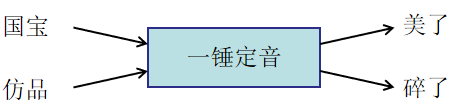
\includegraphics[width=.55\textwidth]{微信图片_20200606153824.png}
    \caption{“一锤定音”节目流程}
    \label{fig:my_label_1}
\end{figure}
我们的目标是成为高水平的可以做“以假乱真”的高质量仿品的大师,有如下两个要求:

1. 鉴赏专家的水平足够高。

2. 作假的水平足够高。

国宝是古人做的,静态的,不可能发生变化的。而工艺品和作假的水平是变化的。三者中,国宝是静态的,其他的都是可变化的。

有可能有的同学会迷惑,这和生成模型之间有什么关系呢?如果一个仿品可以和国宝做的一模一样,不就相当于学到了真实数据的分布,可以完全模拟出真实数据。下一步则是,想办法将模型用数学语言描述。

\section{数学语言描述}
\subsection{模型表示}
工艺大师和鉴赏专家的水平会不断的提高,最终我们会培养一个高水平的工艺大师和一个高水平的鉴赏家。而最终的目的是培养一个高水平的工艺大师,而不是一个高水平的鉴赏家。鉴赏家只是衍生品,最终将达到两个目的,1. 足够的以假乱真;2. 真正的专家看不出来。

所以,我们需要加一些feedback,令工艺大师收到专家给出的反馈。并且鉴赏大师也要从工艺大师那里知道真实的情况来提升自己的水平。如下图所示:
\begin{figure}[H]
    \centering
    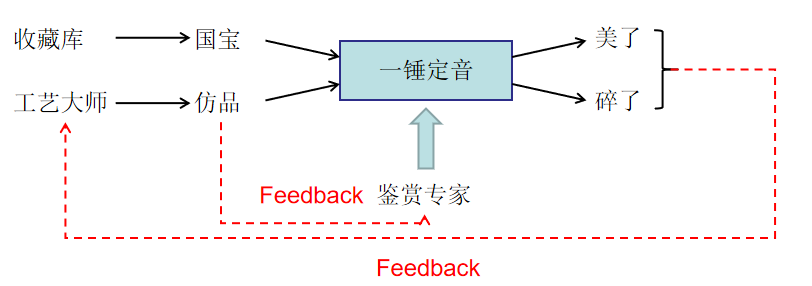
\includegraphics[width=.85\textwidth]{微信图片_20200606165431.png}
    \caption{GAN的详细流程}
    \label{fig:my_label_1}
\end{figure}
我们可以将古人,视为$P_{\text{data}}$,$\{x_i\}_{i=1}^N$,实际就是经验分布,通常我们将经验分布视为数据分布。

工艺品,是从一个模型分布$P_g$采样出来的,$P_g(x;\theta_g)$。我们本身不对$P_g$建模,而是用一个神经网络来逼近$P_g$。假设$z$来自一个简单分布,并增加噪声,$z\sim P_z(z)$。其中,$x=G(z;\theta_g)$
\begin{figure}[H]
    \centering
    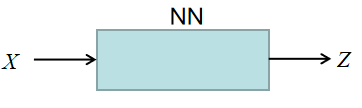
\includegraphics[width=.35\textwidth]{微信图片_20200606171236.png}
    \caption{工艺大师网络结构图}
    \label{fig:my_label_1}
\end{figure}
鉴赏专家输出的是一个概率分布,同样也是一个神经网络,$D(x,\theta_d)$,其代表的是输入一个物品,判断其为国宝的概率。$D\to 1$是国宝,$D\to 0$是工艺品。模型如下所示:
\begin{figure}[H]
    \centering
    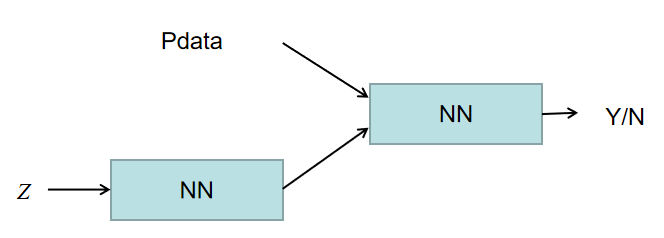
\includegraphics[width=.65\textwidth]{微信图片_20200606173145.png}
    \caption{模型的数学表示}
    \label{fig:my_label_1}
\end{figure}

我们的目标有两个:

\textbf{1. 高专家:}
高水平的专家可以正确的分辨国宝和赝品。

\begin{equation}
    \left\{
    \begin{array}{ll}
      \text{if $x$ is from $P_{data}$ then $D(x)$ $\uparrow$ } & \\
      \text{if $x$ is from $P_{g}$ then $1-D(x)$ $\downarrow$ } & \\
    \end{array}
    \right.
\end{equation}

其中,我们将用对数似然函数的形式来进行表达。而$1-D(x)$中的$x$是来自$G(z)$的,那么,高专家部分的目标函数为:
\begin{equation}
    \max_D \underbrace{\mathbb{E}_{x\sim P_{data}}[\log D(x)]}_{\frac{1}{N} \sum_{i=1}^N \log D(x_i)} +  \mathbb{E}_{x\sim P_{z}}[\log (1-D(G(z)))]
\end{equation}

\textbf{2. 高大师:}
高水平的大师的目的就是要造成高水平的鉴赏专家分辨不出来的工艺品,可以表示为:
\begin{equation}
    \text{if $x$ is from $P_g$ then $\log(1-D(G(z)))$ $\uparrow$}
\end{equation}
此目标表达为数学语言即为:
\begin{equation}
    \min_G \mathbb{E}_{z\sim P_g}[\log(1-D(z))]
\end{equation}
根据图2中的feedback流向,我们可以了解到,先优化鉴赏专家,再优化工艺大师。总优化目标是:
\begin{equation}
    \min_G \max_D \mathbb{E}_{x\sim P_{data}}[\log D(x)] + \mathbb{E}_{x\sim P_{z}}[\log (1-D(G(z)))]
\end{equation}
\subsection{小结}
GAN模型本身思想很简单,难点主要在于学习$\theta_g,\theta_d$。GAN中没有直接面向$P_g$建模,而是从一个可微的NN中采样来逼近$D_g(x;\theta_g)$。不是直接面对分布,而是绕过复杂的求解过程来近似。我们之前分析过,如果用NN来近似概率分布,这叫Implicit Density Model。下一步则是考虑如何求解全局最优解。

\section{全局最优解}
GAN模型表示汇总如下所示:
\begin{figure}[H]
    \centering
    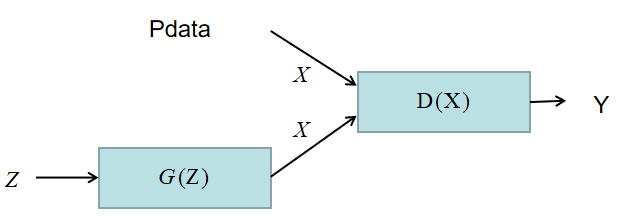
\includegraphics[width=.65\textwidth]{微信图片_20200606182808.png}
    \caption{GAN的数学表示}
    \label{fig:my_label_1}
\end{figure}

$P_{data}$:$\{x_i\}_{i=1}^N$

$P_g(x;\theta_g)$:generator,$G(z;\theta_g)$

$y|x$:discriminater,$P(y=1|x)=D(x)$,$P(y=0|x)=1-D(x)$

$G(z;\theta_g)$和$D(x;\theta_d)$是两个多层感知机。GAN就是这样采用对抗学习,其最终目的就是$P_g = P_{data}$。目标函数中,记:
\begin{equation}
    V(D,G) = \mathbb{E}_{x\sim P_{data}}[\log D(x)] + \mathbb{E}_{x\sim P_{z}}[\log (1-D(G(z)))]
\end{equation}
最终的目标是令$P_g = P_{data}$,而$P_g $中的参数为$\theta_g$。在之前的极大似然估计思想中,
\begin{equation}
    \theta_g = \arg\max_{\theta_g} \sum_{i=1}^N \log P_g(x_i)
\end{equation}
而对$P_g(x_i)$比较复杂,通常采用EM算法和VI来进行近似,通过推导可以得出,最后的目标为:
$$\arg\min_{\theta_g} \text{KL}(P_{data}\|P_g)$$

~\\

对公式(5)的求解过程可以分成两步,而第一步为求解过程为fixed G,求解$\max_D V(G,D)$
\begin{equation}
    \begin{split}
        \max_D V(D,G) = & \int P_{\text{data}} \log D dx + \int P_g \log(1-D) dx \\
        =& \int (P_{\text{data}} \log D dx + P_g \log(1-D)) dx
    \end{split}
\end{equation}

通过求偏导来计算最优解:
\begin{equation}
    \begin{split}
        \frac{\partial (V(D,G))}{\partial D} = & \frac{\partial}{\partial D} \int \left[ P_{\text{data}} \log D dx + P_g \log(1-D) \right]dx \\
        = &  \int \frac{\partial}{\partial D} \left[ P_{\text{data}} \log D dx + P_g \log(1-D) \right]dx \\
        = & 0 \\
    \end{split}
\end{equation}
这一步的推导利用了微积分的基本定理,得到:
$$
\int P_{\text{data} }\cdot \frac{1}{D} + P_g \frac{-1}{1-D} dx = 0
$$
恒成立,所以有:
\begin{equation}
    D^\ast = \frac{P_{\text{data}}}{P_{\text{data}} + P_{g}}
\end{equation}
第二步,将求解的是:
\begin{equation}
    \begin{split}
        \min_G \max_D V(D,G) = & \min_G V(D^\ast,G) \\
        = & \min_D \mathbb{E}_{x\sim P_{\text{data}}} \left[   \log \frac{P_{\text{data}}}{P_{\text{data}} + P_{g}}\right] + \mathbb{E}_{x\sim P_{g}} \left[   \log \frac{P_g}{P_{\text{data}} + P_{g}}\right]
    \end{split}
\end{equation}
观察$\mathbb{E}_{x\sim P_{\text{data}}} \left[   \log \frac{P_{\text{data}}}{P_{\text{data}} + P_{g}}\right]$会发现这很像一个KL散度,但是$P_{\text{data}} + P_{g}$不是一个概率分布。所以,通过$\frac{P_{\text{data}} + P_{g}}{2}$来将其转换为一个概率分布。那么有,
\begin{equation}
\begin{split}
    \min_G \max_D V(D,G) = & \min_G \mathbb{E}_{x\sim P_{\text{data}}} \left[   \log \frac{P_{\text{data}}}{\frac{P_{\text{data}} + P_{g}}{2}} \cdot \frac{1}{2}\right] + \mathbb{E}_{x\sim P_{g}} \left[   \log \frac{P_g}{\frac{P_{\text{data}} + P_{g}}{2}} \cdot \frac{1}{2}\right] \\
    = & \min_G \text{KL}\left[ P_{\text{data}} \| \frac{P_{\text{data}} + P_{g}}{2} \right] + \text{KL}\left[ P_{g} \| \frac{P_{\text{data}} + P_{g}}{2} \right] - \log 4 \\
    \geq & - \log 4
\end{split}
\end{equation}

当且仅当$P_{\text{data}}  = P_{g} = \frac{P_{\text{data}} + P_{g}}{2}$时,等号成立。此时,$P^\ast_g = P_d,P^\ast_d = \frac{1}{2}$。很显然,大家想一想就知道,生成器模型分布最好当然是和数据分布是一样的,而此时判别器模型真的和假的都分不出,输出都是$\frac{1}{2}$。

\section{总结}
本章主要描述了什么是GAN,GAN是一种生成模型。其实,以前我对GAN的理解,只是它可以画图,生成和真实数据一样的图,并不知道它有什么用。通过系统的学习,我现在对生成模型的意义有了不一样的认识。本章主要介绍的是GAN的模型意义和模型表示,以及简单的求解过程。实际上,GAN中有很多很多的问题,这只是最基础的版本,介绍简单的思想而已,希望可以抛转引玉。


\end{document}
